\section{Experimental Setup}

In this work, we will build OSVTF based on ViT [4] configuration.The output feature map of The FPN Fusion has the same number of feature dimensions as the number of channels in the first layer of the scaled feature convolution map.The encoder contains 8 transformer encoder layers ($L\times 8$) and each MHSA in the encoder layer contains 12 heads ($M=12$), 768 features ($D=768$), and a sliding window of size $4\times 4$ steps of $2$ ($P=4,S=2$).The number of feature dimensions, the number of heads in the Decoder part, the MHSA and the CMHA, are kept the same as in the parts of the encoder, and the number of heads is kept the same as in the parts of the encoder, and the number of heads is the same as the number of channels of the first layer scale feature convolutional map in the encoder layer, and the number of channels of the first layer scale feature convolutional map in the encoder layer is the same as in the first layer scale feature convolutional map. weighted-sum's the number of feature dimensions for patch embeddings mapping is set to 512 ($d_P=512$).

On the loss function, the partial settings $n=0.3,m=0.9,\alpha_1=0.6,\alpha_2=0.8$ and $\overline{K}=\overline{V}=10$ are followed for TransOSV.The hyper-parameters are set to $\lambda_1=0.5,\lambda_2=1.0,\lambda_3=0.5,\lambda_4=2.0,\xi=0.2$.On the optimizer, all experiments are On the optimizer, all experiments are conducted on 2 NVIDIA 3080 GPUs and the total batch size is set to be 16.

\section{Metrics}

In terms of evaluation metrics, unlike conventional binary classification tasks, the offline handwritten signature verification task requires special attention to NEGATIVE samples, and therefore standard metrics in biometric and signature verification tasks [7] are used to evaluate the performance of OSVTF, i.e., False Rejection Rate (FRR), False Acceptance Rate (FAR) and Equal Error Rate (EER). In a conventional binary classification task, the concept of confusion matrix [6] is used to count the number of sample labels and predicted labels in the format of Table \ref{tab:cm}.

\begin{table}[htbp]
\caption{Confusion Matrix}  
\begin{center}
\begin{tabu} to 0.8\textwidth{X[3, c]X[3, c]X[3, c]}  
%0.8\textwidth   为设置表格宽度  
%X[c]      表示这一列居中,所占比例为1,相当于X[1,c]  
%X[3,c]   表示这一列居中,所占比例为3,这列的宽度是X[c]列的3倍  
\toprule
predicted Label / raw label & $\hat{y}=0$ (positive) & $\hat{y}=1$ (negative)\\
\midrule
$y=0$ &  True Positive (TP) & False Negative (FN) \\
$y=1$ & False Positive (FP) & True Negative (TN) \\
\bottomrule
\end{tabu}
\end{center}
\label{tab:cm}
\end{table}

This leads to the following formula for FRR, and FAR:
\begin{equation}
\label{eq21}
\begin{aligned}
	\text{FRR}=\frac{\text{FN}}{\text{FN}+\text{TP}} \\
	\text{FAR}=\frac{\text{FP}}{\text{FP}+\text{TN}}
\end{aligned}
\end{equation}
The EER is calculated using several thresholds and distances for comparison, if the feature distance of the sample pair is greater than the threshold, then its category is FORGED, otherwise it is GENUINE.This work will calculate the distance based on the model features of the sample pairs of the batch data during the training process, and based on the distance minima and maxima of the sample pairs in order to set a number of thresholds, so that the FAR and FRR are automatically calculated for the current batch for each threshold value. FAR and FRR are calculated for each threshold and when the difference between FAR and FRR is the smallest, then FRR, FAR for the current threshold are output simultaneously and EER is calculated as follows:

\begin{equation}
\label{eq22}
	\text{EER} = \frac{\text{FRR}+\text{FAR}}{2}	
\end{equation}
	
As a result, the experimental phase will be based on the four evaluation indexes of ACC, FRR, FAR and EER to comprehensively assess the model performance.

\newpage
\section{Dataset}

BHSig-B and BHSig-H. Both datasets are published by Indian Institute of Technology Guwahati (IIT Guwahati) [3] dataset of handwritten signatures in Bengali and Hindi. Where BHSig-B contains Bengali handwritten signatures of 100 authors and BHSig-H contains Hindi handwritten signature images of 160 authors. Each user handwritten signature has signed 24 authentic and 30 forged signatures.
CEDAR. This dataset is an English handwritten signature dataset developed and published by Center of Excellence for Document Analysis and Recognition [28]. It contains 55 handwritten signatures of authors in English. Each user signed 24 authentic and 24 forged signatures by hand.

\section{Results Analysis}

\subsection{Writer-Independent Results}

On the WI task, OSVTF takes the Euclidean distance method to calculate the distance between two features to determine whether the signature is forged or not, in order to evaluate whether OSVTF outperforms the past models in possessing offline handwritten signature verification performance. The initial stage is validated on BHSig-B and BHSig-H, which are consistent with the past algorithms, by dividing the 100 authors of BHSig-B into training and testing sets according to the ratios of 50:50 and 80:20 for 100 authors, and dividing the 160 authors of BHSig-H into training and testing sets according to the ratio of 100:60 for 160 authors. The preliminary experimental results obtained are shown in Table \ref{tab:wi}.

\begin{table}[htbp]
\caption{BHSig-B and BHSig-H dataset WI signature verification performance comparison}  
\begin{center}
\begin{tabu} to 0.8\textwidth{X[3, l]X[2, l]X[2, l]X[2, l]}  
%0.8\textwidth   为设置表格宽度  
%X[c]      表示这一列居中,所占比例为1,相当于X[1,c]  
%X[3,c]   表示这一列居中,所占比例为3,这列的宽度是X[c]列的3倍  
\toprule
Model & FRR & FAR & EER \\
\midrule
BHSig-B \\
\midrule
50/50 \\
SigNet [30] & 13.89 & 13.89 & 13.89 \\
CaP [24] & 3.96 & 3.96 & 3.96 \\
IDN [40]	& 5.24 & 4.12 & - \\
InceptionSVGNet [39]	& 2.22 & 3.88 & - \\
TransOSV [38] & 9.90 & 9.90 & 9.90 \\
TransOSV [Ours] & 12.41 & 12.41 & 12.41 \\
OSVTF [Ours] & 10.72 & 10.85 & 10.79 \\
\midrule
80/20			
DeepHsv[41] & 11.92 & 11.92 & 11.92 \\
TransOSV & 3.56 & 3.56 & 3.56 \\
TransOSV [Ours] & 5.11 & 5.11 & 5.11 \\
OSVTF [Ours] & 4.47 & 4.61 & 4.54 \\
\midrule
BHSig-H 100/60 \\
SigNet [30] & 15.36 & 15.36 & 15.36 \\
IDN [40] & 4.93 & 8.99 & - \\
CaP [24] & 5.97 & 5.97 & 5.97 \\
InceptionSVGNet [39] & 3.33 & 6.38 & - \\
TransOSV [38] & 3.24 & 3.24 & 3.24 \\
TransOSV [Ours] & 4.86 & 4.86 & 4.86 \\
OSVTF [Ours] & 3.86 & 3.94 & 3.90 \\
\bottomrule
\end{tabu}
\end{center}
\label{tab:wi}
\end{table}

Among them, in the BHSig-B dataset, 10.79\% EER for OSVTF at 50:50 ratio and 12.41\% EER for reproduced TransOSV, with a difference of about 15.01\%, and 4.54\% EER for OSVTF at 80:20 ratio and 5.11\% EER for reproduced TransOSV, with a difference of about 12.56\%. In the BHSig-H dataset, 4.86\% EER for reproduced TransOSV, 3.90\% EER for OSVTF, a difference of about 24.62\%. The OSVTF performance on the WI task outperforms the TransOSV performance by about 17\%.

\subsection{Writer-Dependent Results}

On the WD task, in addition to the experiments on the model with the addition of multiscale fusion features, a classifier for the deep learning traditional image classification task (GAP classifier) was added to verify if it is a better fit compared to the SVM's classifier for the model with multiscale fusion features. Therefore, the 80:20 ratio of BHSig-B and BhSig-H were validated and the results are shown in Table \ref{tab:wd}.

\begin{table}[htbp]
\caption{BHSig-B and BHSig-H dataset WD signature verification performance comparison}  
\begin{center}
\begin{tabu} to 0.8\textwidth{X[3, l]X[2, l]X[2, l]X[2, l]}  
%0.8\textwidth   为设置表格宽度  
%X[c]      表示这一列居中,所占比例为1,相当于X[1,c]  
%X[3,c]   表示这一列居中,所占比例为3,这列的宽度是X[c]列的3倍  
\toprule
Model & FRR & FAR & EER \\
\midrule
BHSig-B 80/20 \\
TransOSV [Ours] & 3.78 & 3.78 & 3.78 \\
OSVTF [SVM] & 2.74 & 2.80 & 2.77 \\
OVSTF [GAP] & 2.05 & 2.21 & 2.13 \\
\midrule
BHSig-H 100/60 \\
TransOSV [Ours] & 4.23 & 4.23 & 4.23 \\
OSVTF [SVM] & 3.17 & 3.21 & 3.19 \\
OVSTF [GAP] & 2.67 & 2.69 & 2.68 \\
\bottomrule
\end{tabu}
\end{center}
\label{tab:wd}
\end{table}

Also using SVM as a classifier, in the experimental results on the BHSig-B dataset, OSVTF 2.77\% EER decreased by 36.46\% compared to TransOSV's 3.78\% EER, and in the experimental results on the BHSig-H dataset, OSVTF 3.17\% EER decreased compared to TransOSV's 4.23\% EER by 33.44\%. The OSVTF performance on the WD task outperforms the TransOSV performance by about 34.95\%. On the experimental results of different classifiers, OSVTF 2.13\% EER of BHSig-B taking GAP classifier is better than OSVTF 2.77\% EER taking SVM classifier; OSVTF 2.68\% EER of BHSig-H taking GAP classifier is better than OSVTF 3.19\% EER taking SVM classifier. on the overall WD task, OSVTF of OSVTF also taking SVM classifier outperforms TransOSV by about 34.95\%, and can improve by another 19.03\% when taking GAP classifier.

\section{Ablation Experiments}

In the above experimental results, it is shown that OSVTF with the addition of multi-scale fusion features improves the performance on the WI task by about 17\% and on the WD task by about 35\% (and by about 45\% when GAP classification is taken) compared to TransOSV. In this part of the work, ablation experiments will be conducted for the multiscale fusion features, Conv-Module downsampling method, decoder multicast optimization, and sparsity loss in order to verify the performance enhancement of each part for OSVTF, and the obtained WI experimental results are shown in Table \ref{tab:ae}.


\begin{table}[htbp]
\caption{WI ablation experiments}  
\begin{center}
\begin{tabu} to 0.9\textwidth{X[4.5,c]X[2,c]X[2,c]X[2,c]X[2,c]X[9, l]X[9, l]X[8, l]}  
%0.8\textwidth   为设置表格宽度  
%X[c]      表示这一列居中,所占比例为1,相当于X[1,c]  
%X[3,c]   表示这一列居中,所占比例为3,这列的宽度是X[c]列的3倍  
\toprule
Model & $\mathcal{F}$ & $\mathcal{C}$ & $\mathcal{P}$ & $\mathcal{L}_{spa}$ & BHSig-B(80/20) & BHSig-H(100:60) & CEDAR(50:5) \\
\midrule
TransOSV &  &  &  &  & 5.11 & 4.86 & 5.94 \\
Baseline & √ &  &  &  & 4.71 & 4.39 & 5.40 \\
& & √ &  &  & 4.83 & 4.55 & 5.67 \\
&  &  & √ &  & 4.92 & 4.76 & 5.61 \\
& √ & √ & √ &  & 4.64 & 4.21 & 5.21 \\ 
OSVTF & √ & √ & √ & √ & 4.54 & 3.90 & 4.75 \\
\bottomrule
\end{tabu}
\end{center}
\label{tab:ae}
\end{table}

It can be shown that the addition of fusion features of multi-scale feature maps to TransOSV can substantially reduce the model misclassification rate. The Conv-Module with downsampling approach (with simultaneous addition of input mapping in the decoder) enhances the abstract representation of features for more complex modeling operations. In the multi-head optimization of the decoder, multiple perspectives are added to focus on the feature vectors, so the model performance is improved. In the sparsity loss training scheme, the distribution of attention in the decoder is slightly weakened, allowing more attention to be paid to individual local features of the signature image.

In the Conv-Module and decoder part of this work, the mapping structure of dimensionality reduction $\to$ dimensionality enhancement is designed to change the whole Conv-Module from the original change in the number of feature dimensions$ D → d_\mathcal{C} \to D$ to $D \times d_\mathcal{C} \times d_\mathcal{C}/2$. In order to comply with this change a "dimensionality enhancement" linear mapping layer is introduced at the Encoder input stage. In order to comply with this change, a "dimension-up" linear mapping layer is introduced at the Encoder input stage. In order to verify the feasibility of the "dimensionality reduction→dimensionality enhancement" mapping structure, a large learning rate and 20 training cycles are set in the experiments on the BHSig-B 50/50 dataset, and the changes in the loss function and evaluation indexes before optimization are shown in Fig. 9, and the changes in the loss function and evaluation indexes after optimization are shown in Figs. \ref{fig:bfloss} and \ref{fig:afloss}.

\begin{figure}[H]
	\centering
	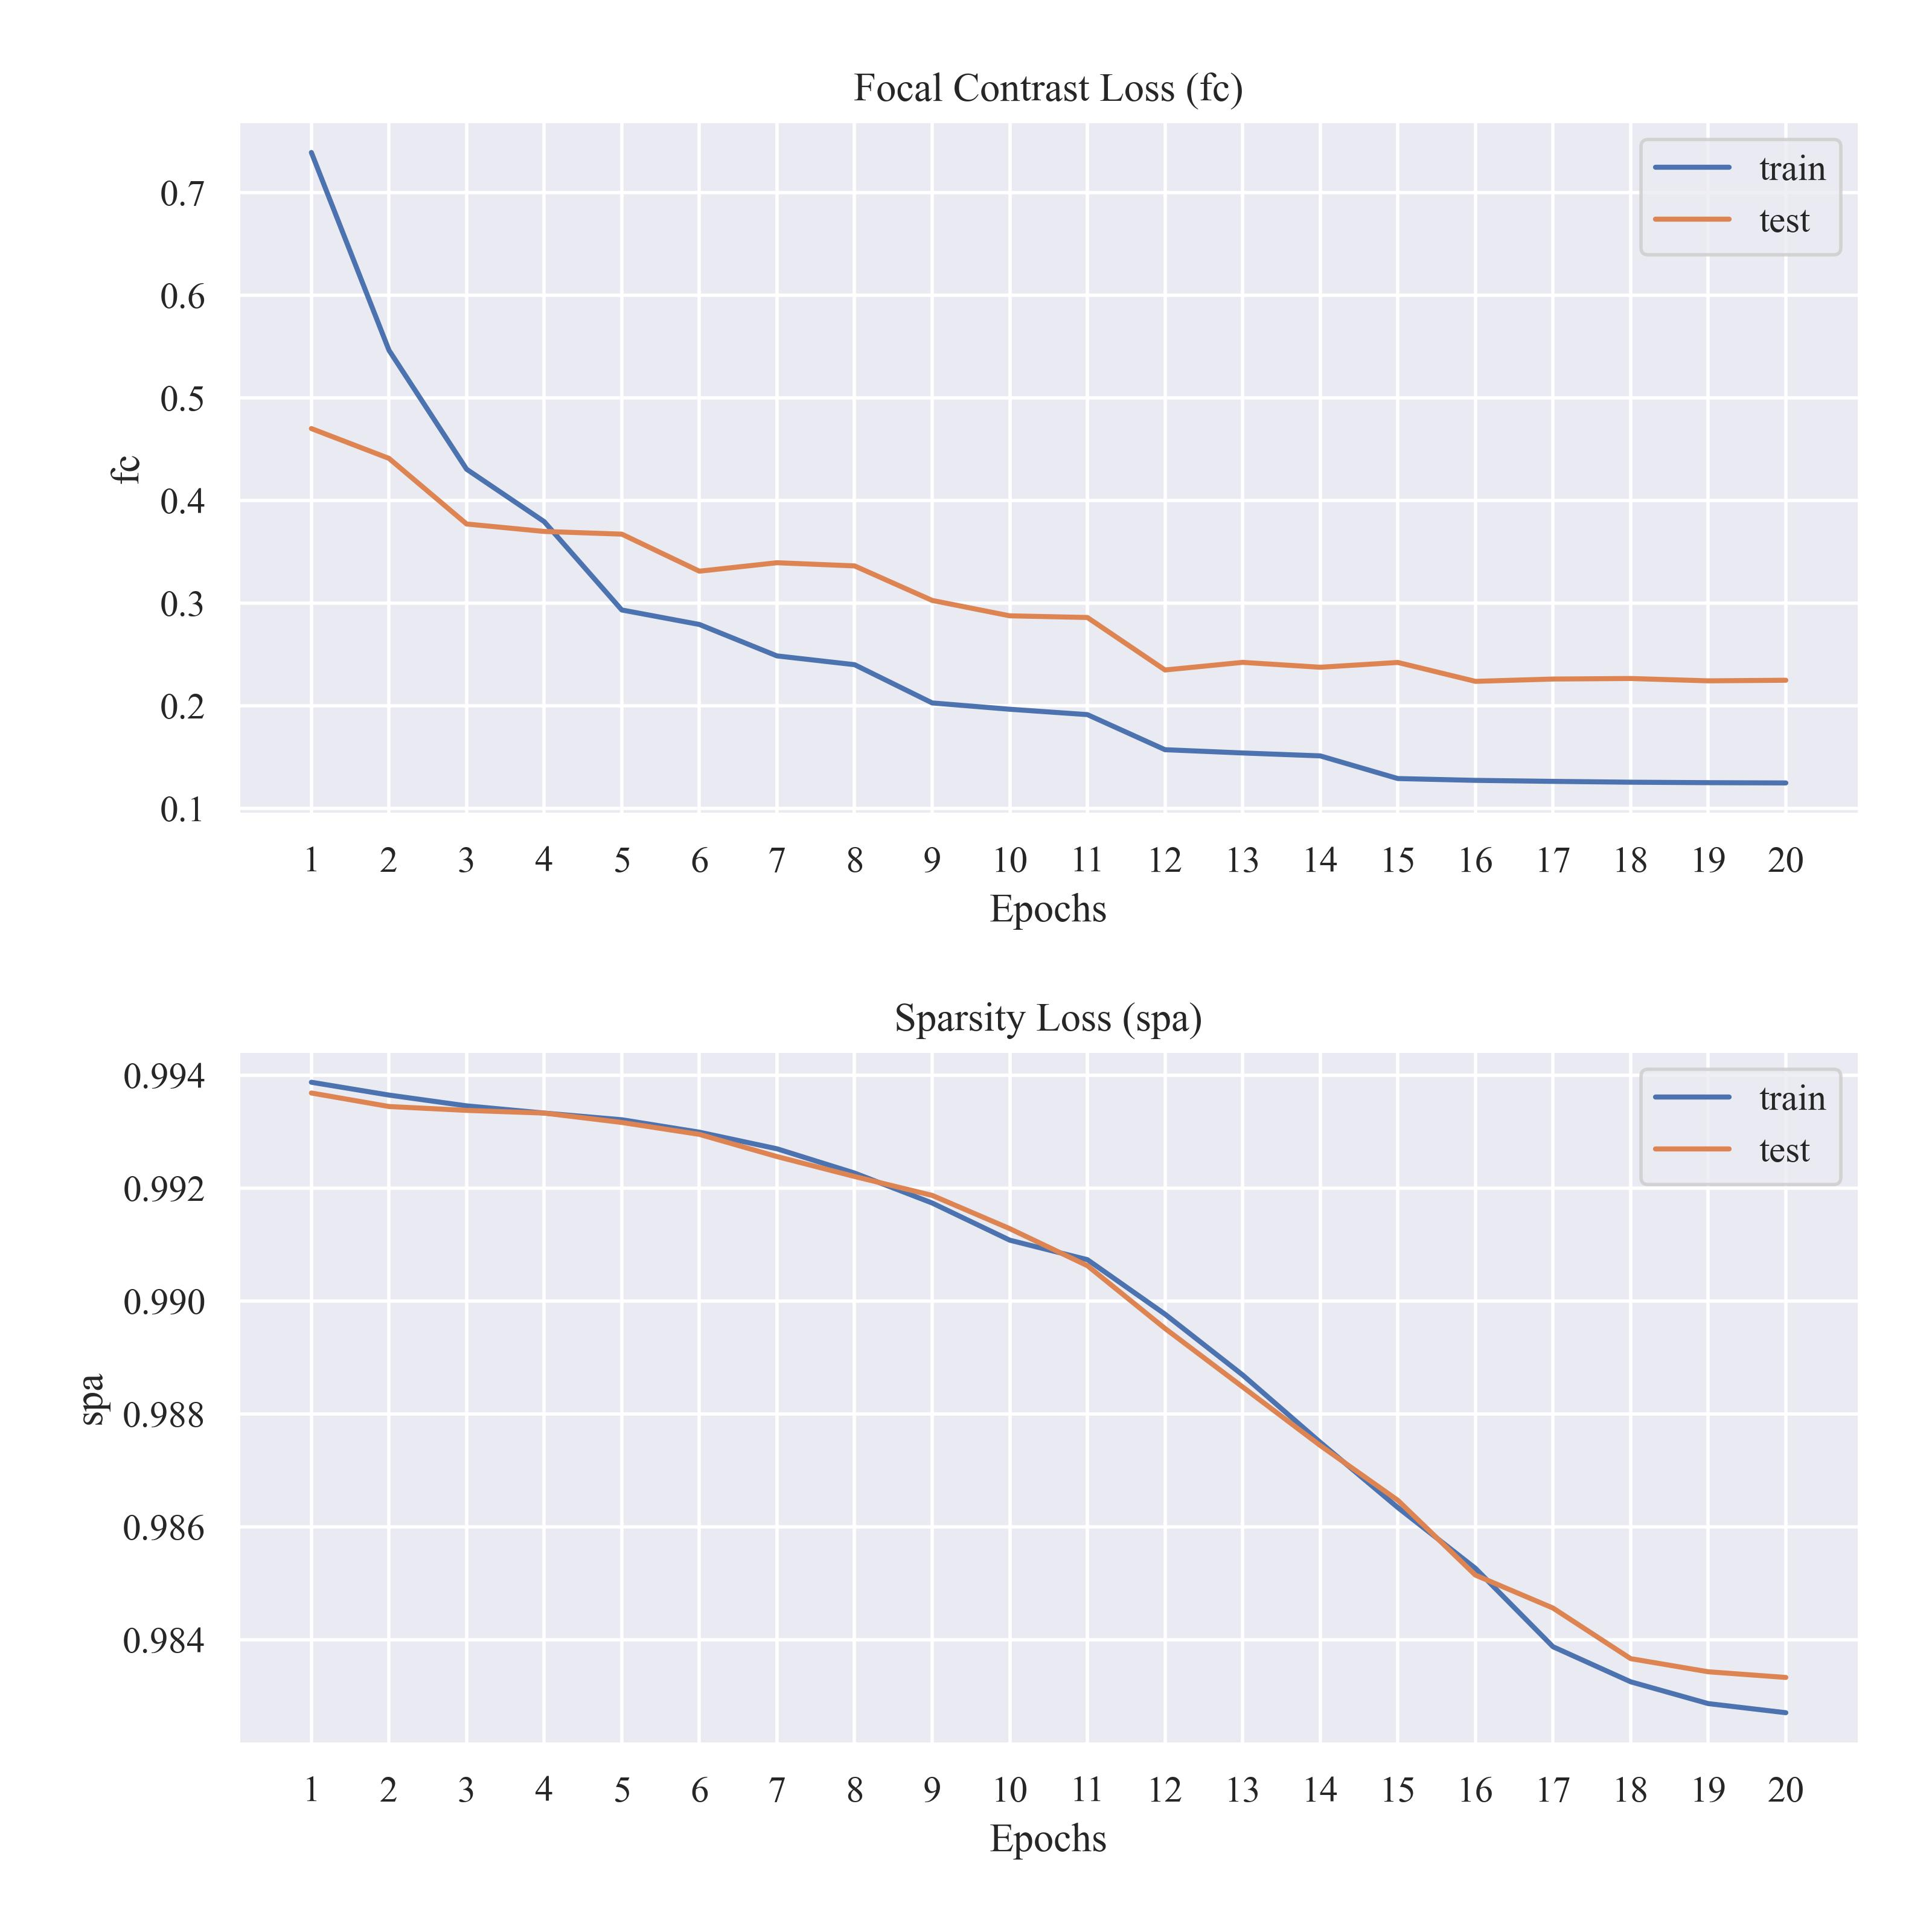
\includegraphics[scale=0.32]{figure/bfloss.jpg}
	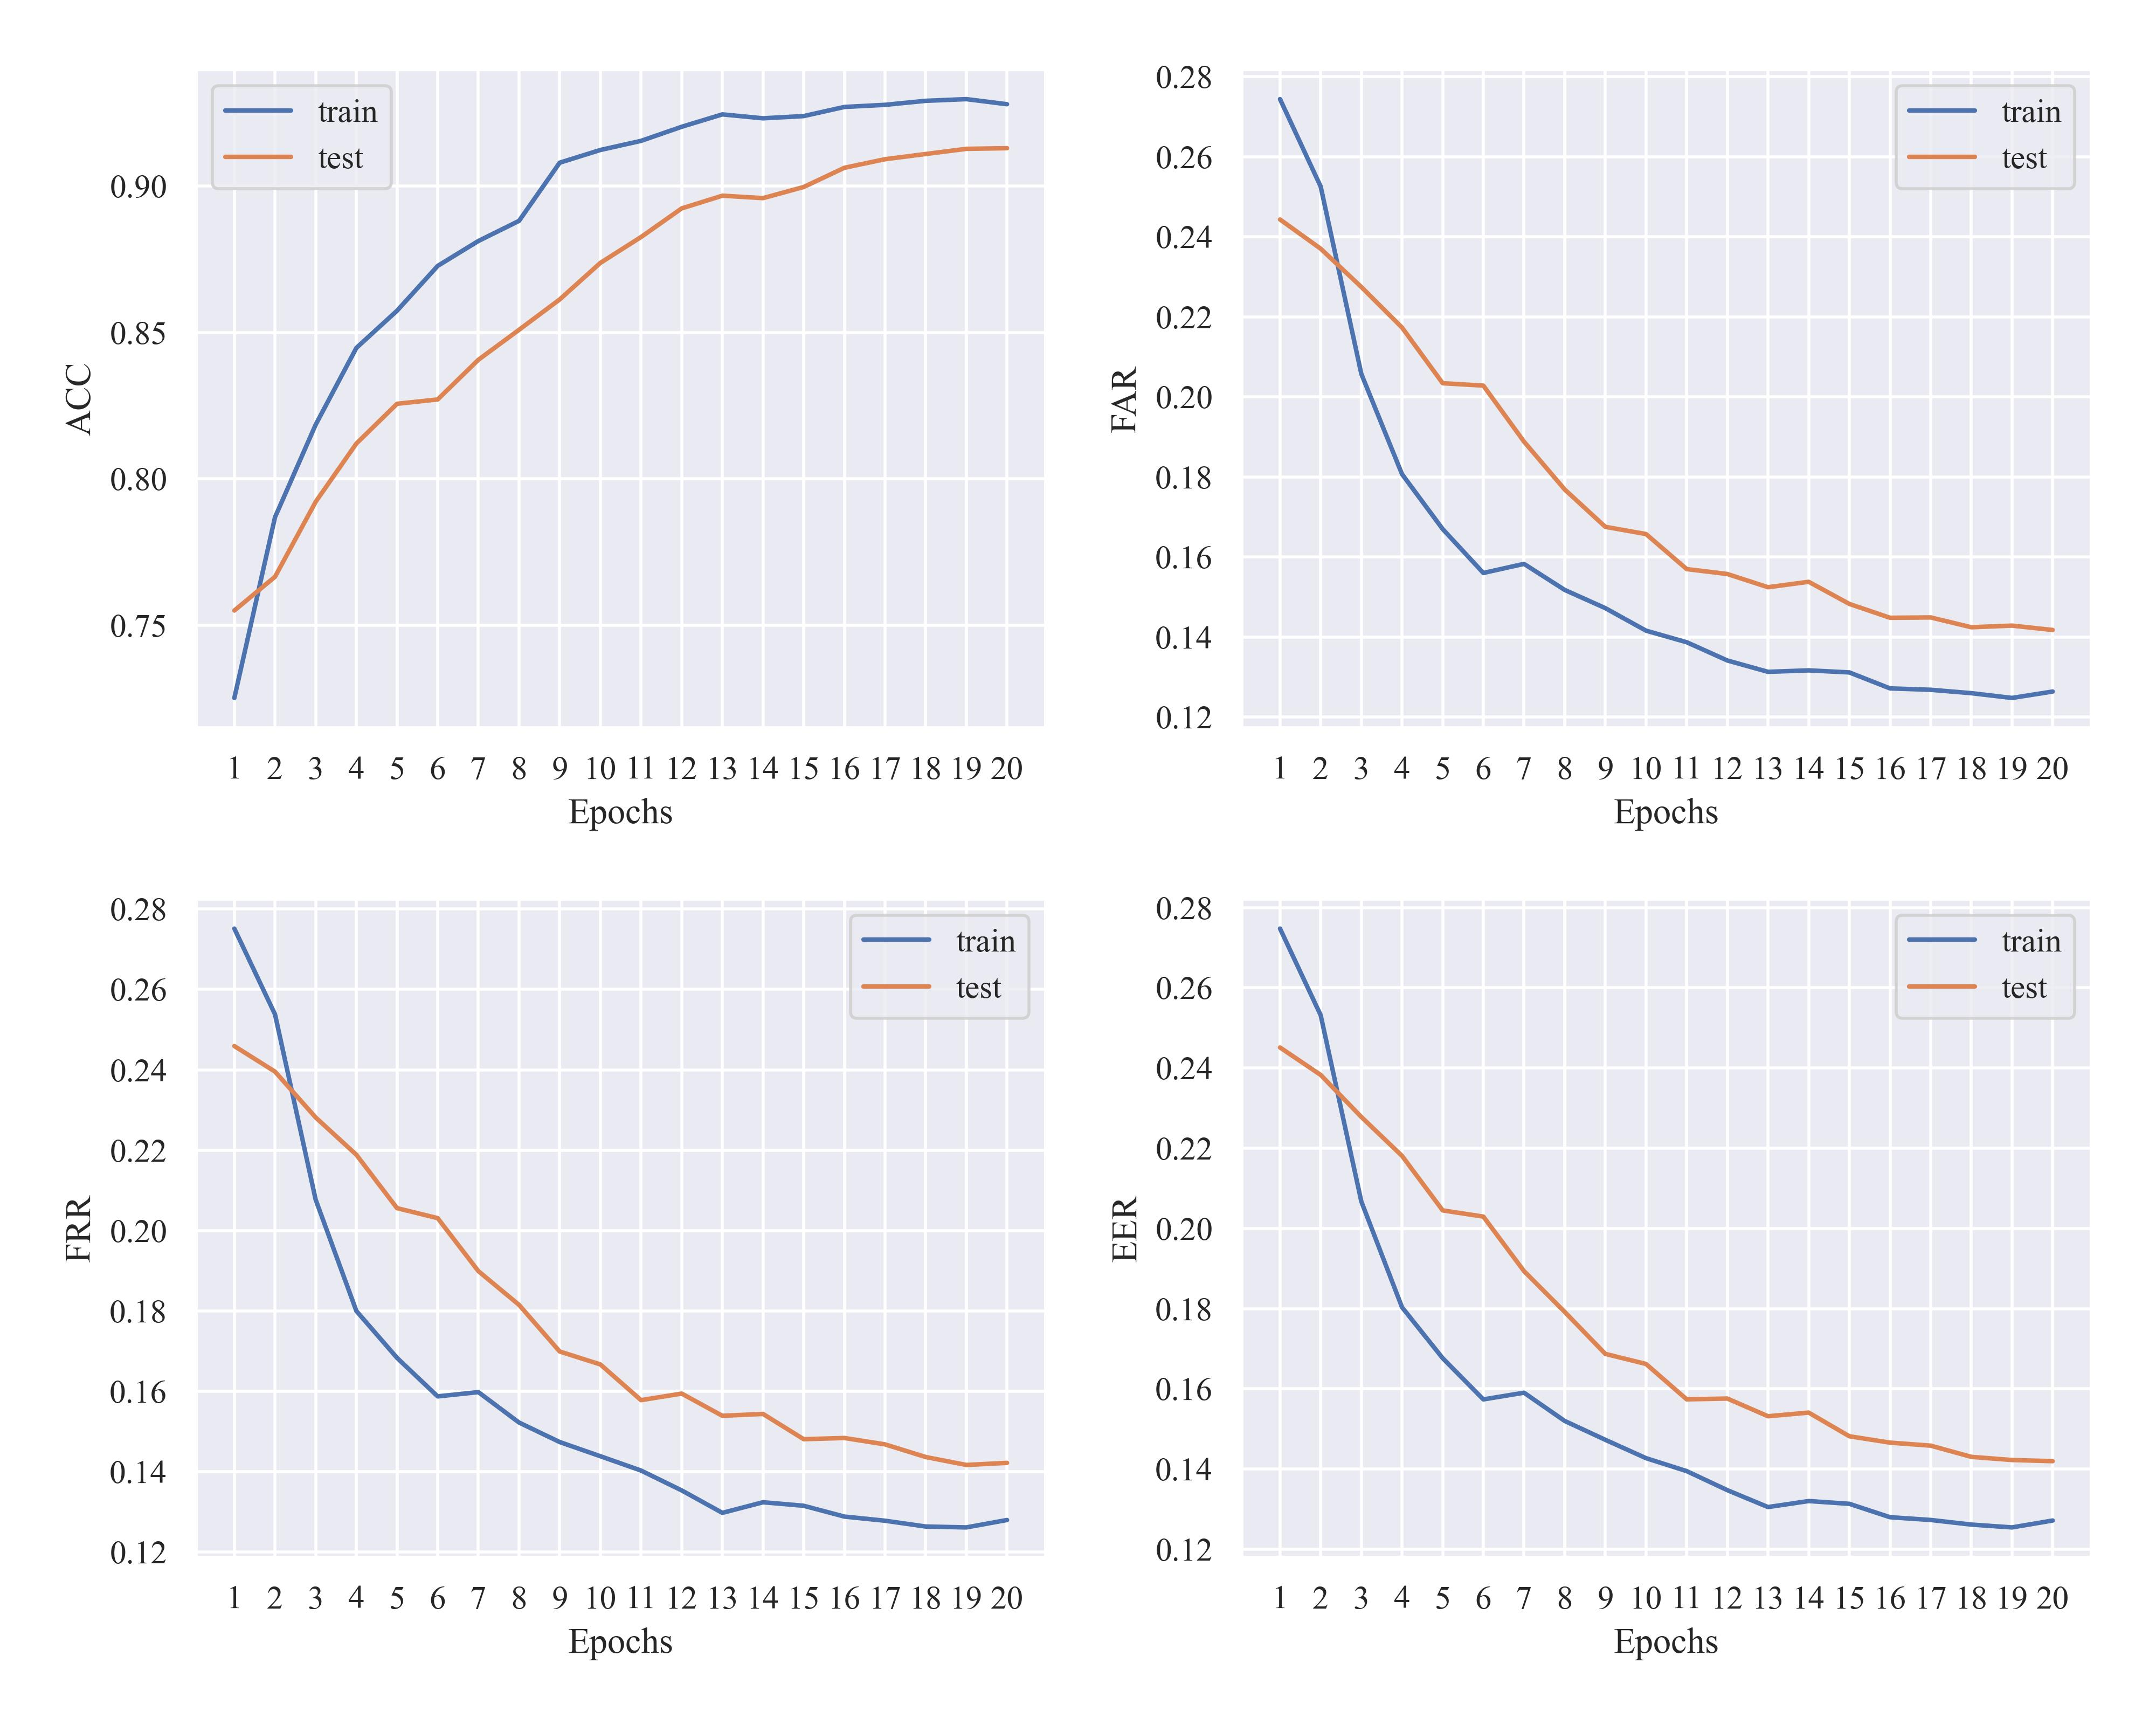
\includegraphics[scale=0.32]{figure/bfmetrics.jpg}
	\caption{Previous Conv-Module loss and metrics diversification}
	\label{fig:bfloss}
  \end{figure}
  
\begin{figure}[H]
\centering
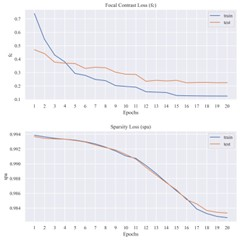
\includegraphics[scale=1]{figure/afloss.jpg}
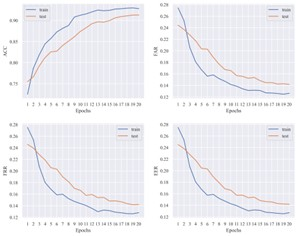
\includegraphics[scale=1]{figure/afmetrics.jpg}
\caption{Optimized Conv-Module loss and metrics diversification}
\label{fig:afloss}
\end{figure}

Based on the results, it can be found that the parameters of the pre-optimization OSVTF start converging at about the 7th or 8th Epoch in the proposed experimental scheme, while the parameters of the optimized OSVTF start converging at about the 3rd or 4th Epoch. This feature processing method of downsampling followed by mapping can effectively accelerate the convergence speed of the model training process. Since the number of features extracted from the intermediate network layer of OSVTF is large, this approach can learn the sensitive part of forged signature features more quickly, and combined with the computation of cross-multiple attention, it further strengthens the learning of the features of the sensitive part of the forged signature, and this approach can reduce a certain number of model parameters, which makes the size of the model weight file become smaller, and the inference speed is accelerated.



% An example of the Algorithm 1.


% \begin{algorithm} 
% 	\SetAlgoVlined 
% 	\caption{identifyRowContext} 
% 	\KwIn{$r_i$, $Backgrd(T_i)$=${T_1,T_2,\ldots, T_n}$ and similarity threshold $\theta_r$} 
% 	\KwOut{$con(r_i)$} 
% 	$con(r_i)= \Phi$\; 
% 	\For{$j=1; j \le n; j \ne i$} 
% 	{ 
% 		float $maxSim=0$\; 
% 		$r^{maxSim}=null$\; 
% 		\While{not end of $T_j$} 
% 		{ 
% 			compute Jaro($r_i,r_m$)\; 

% 		} 
% 		$con(r_i)=con(r_i)\cup {r^{maxSim}}$\; 
% 	} 
% 	return $con(r_i)$\; 
% \end{algorithm}


% There are many sources for Latex editing, see \url{https://latexref.xyz/}.